\chapter{TCP and UDP}\label{tcp-and-udp}

\section{Basics of Layer 4}\label{basics-of-layer-4}

\begin{itemize}
\tightlist
\item
  Provides TRANSPARENT transfer of DATA between END HOSTS (Host To Host
  communication)
\end{itemize}

\begin{figure}
\centering
\pandocbounded{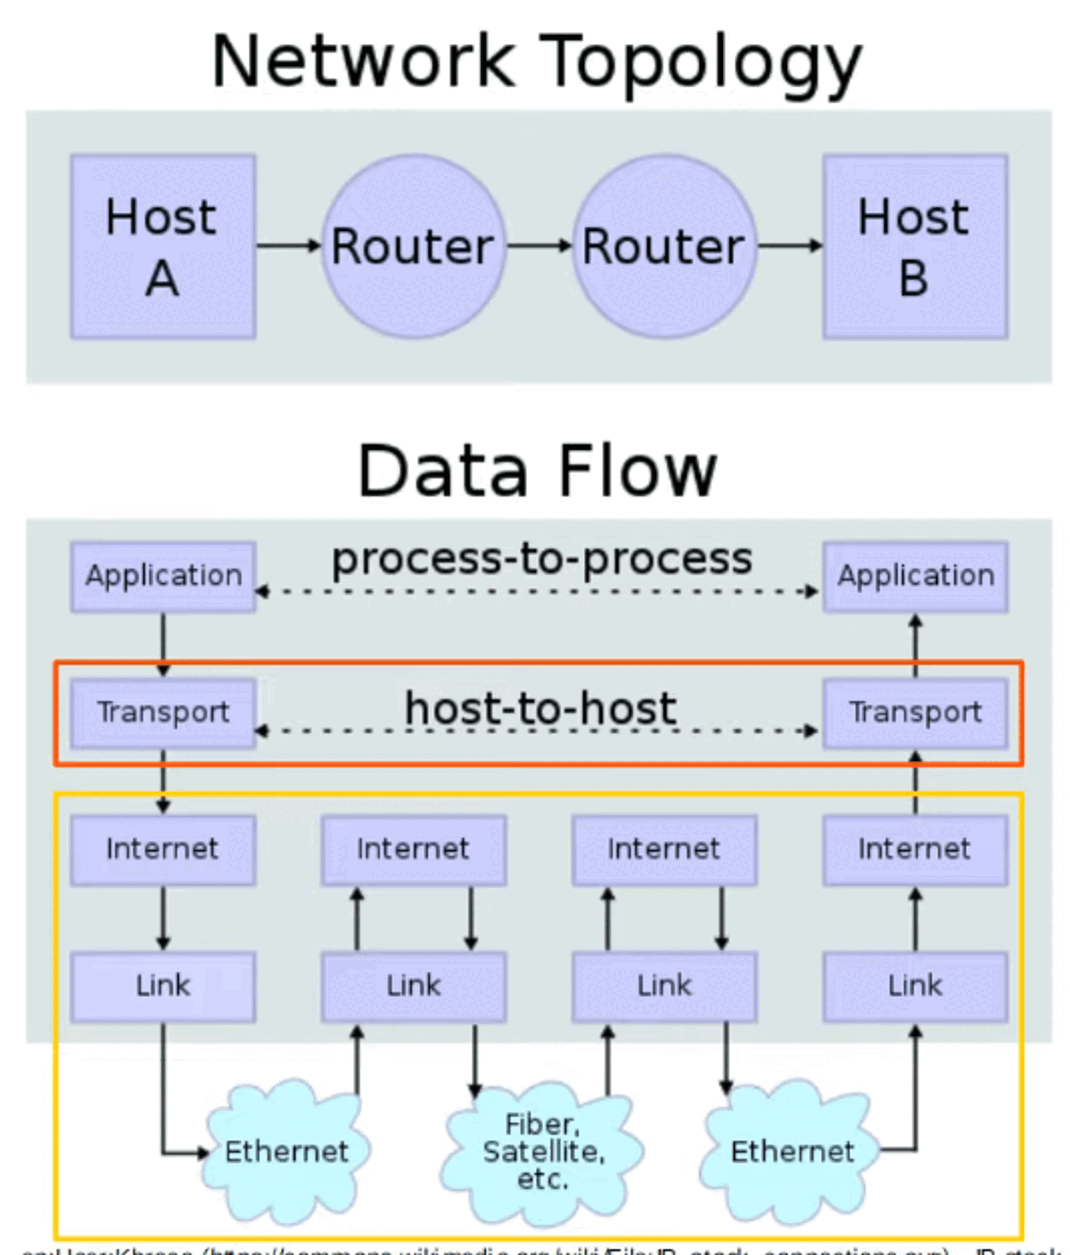
\includegraphics[keepaspectratio,alt={image}]{images/31-tcp-and-udp/img-001.png}}
\end{figure}

\begin{itemize}
\tightlist
\item
  Provides (or DOESN'T provide) various SERVICES to APPLICATIONS:

  \begin{itemize}
  \tightlist
  \item
    Reliable DATA Transfer
  \item
    Error Recovery
  \item
    Data Sequencing
  \item
    Flow Control
  \end{itemize}
\item
  Provides LAYER 4 ADDRESSING (PORT numbers) - NOT the physical
  interfaces / ports on network devices

  \begin{itemize}
  \tightlist
  \item
    IDENTIFY the APPLICATION LAYER protocol
  \item
    Provides SESSION multiplexing
  \end{itemize}
\end{itemize}

WHAT IS A SESSION ?

\begin{itemize}
\tightlist
\item
  A SESSION is an EXCHANGE of DATA between TWO or MORE communicating
  DEVICES
\end{itemize}

\begin{figure}
\centering
\pandocbounded{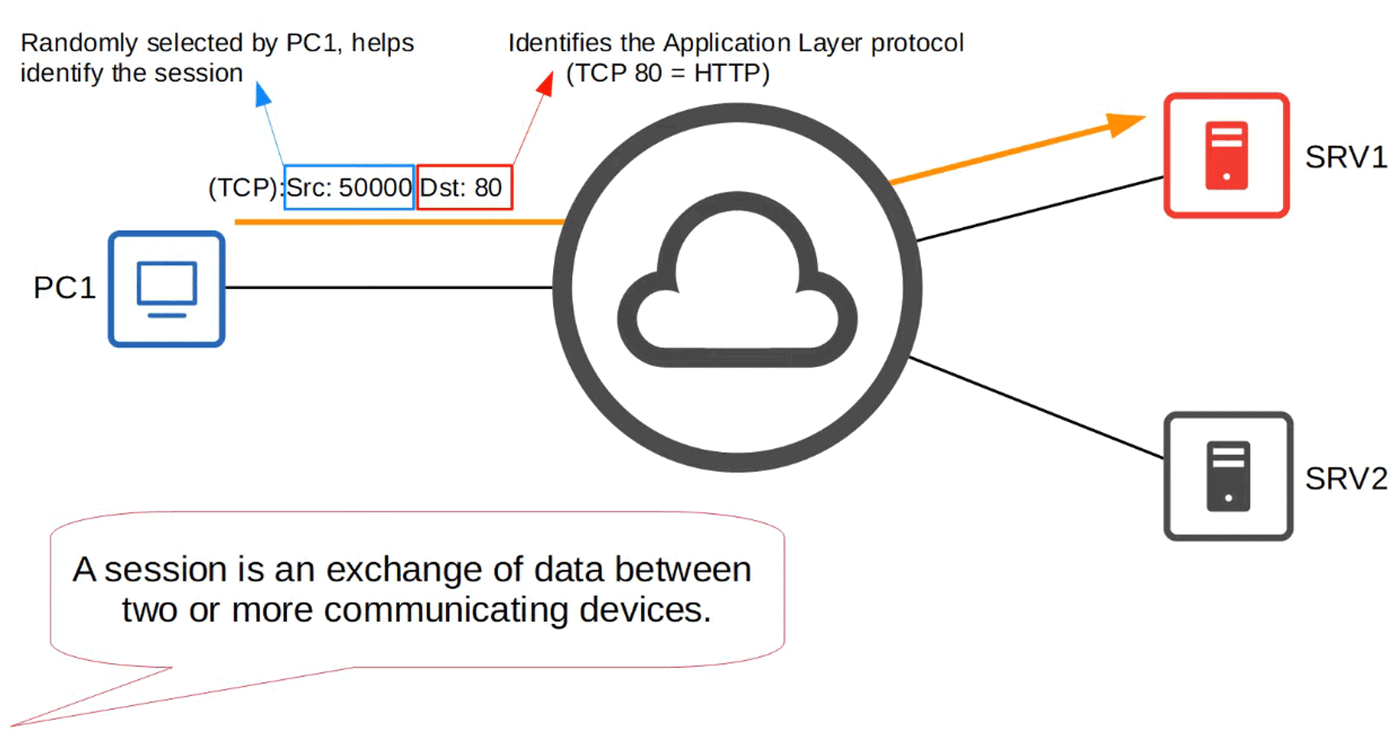
\includegraphics[keepaspectratio,alt={image}]{images/31-tcp-and-udp/img-002.png}}
\end{figure}

The FOLLOWING ranges have been designated by IANA (Internet Assigned
Numbers Authority)

\begin{itemize}
\tightlist
\item
  \textbf{Well-Known} Port Numbers : 0 - 1023
\item
  \textbf{Registered} Port Numbers : 1024 - 49151
\item
  \textbf{Ephemeral} / Private / Dynamic port numbers : 49152 - 65535
\end{itemize}

\begin{figure}
\centering
\pandocbounded{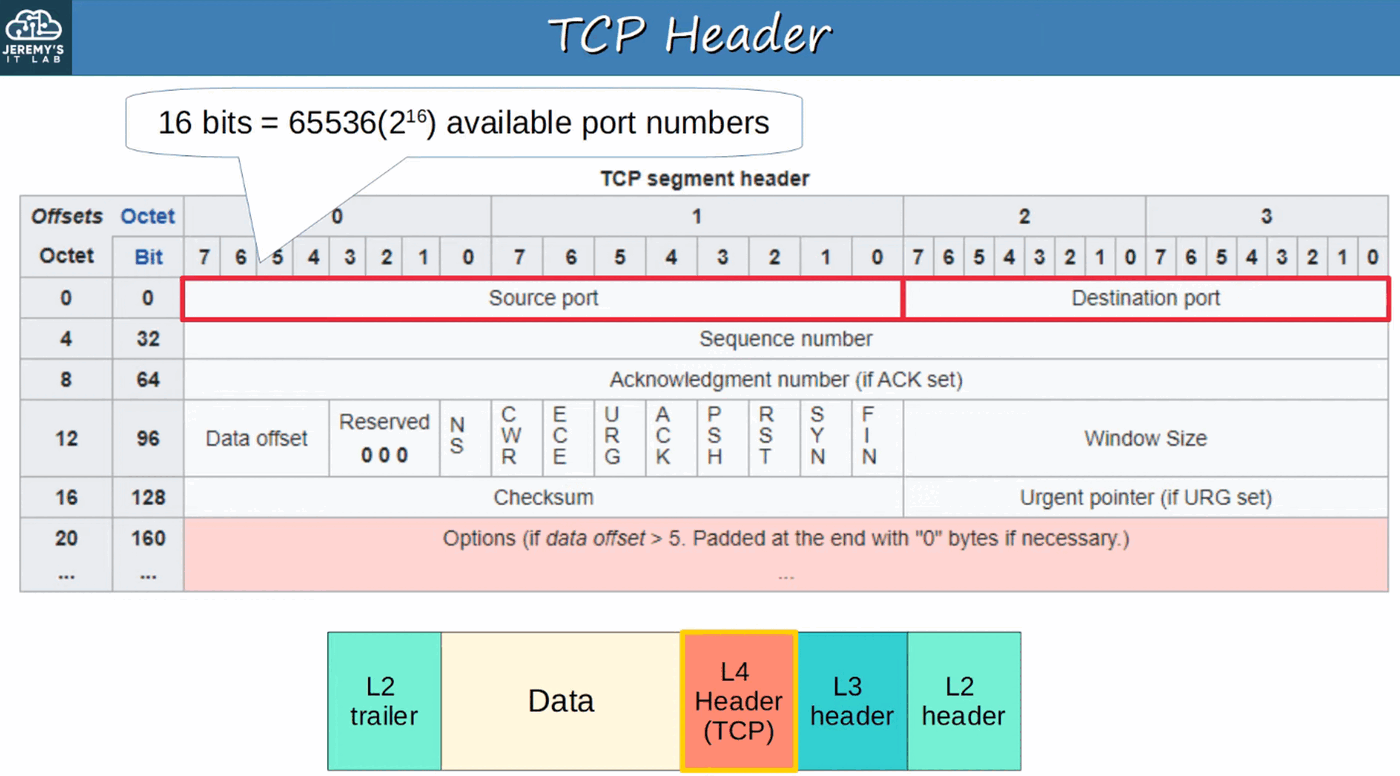
\includegraphics[keepaspectratio,alt={image}]{images/31-tcp-and-udp/img-003.png}}
\end{figure}

\section{TCP (Transmission Control
Protocol)}\label{tcp-transmission-control-protocol}

\begin{itemize}
\tightlist
\item
  A CONNECTION-ORIENTED protocol

  \begin{itemize}
  \tightlist
  \item
    Before actually SENDING DATA to the DESTINATION HOST, the TWO HOSTS
    communicate to establish a CONNECTION. Once the CONNECTION is
    established, DATA exchange begins.
  \end{itemize}
\end{itemize}

\begin{figure}
\centering
\pandocbounded{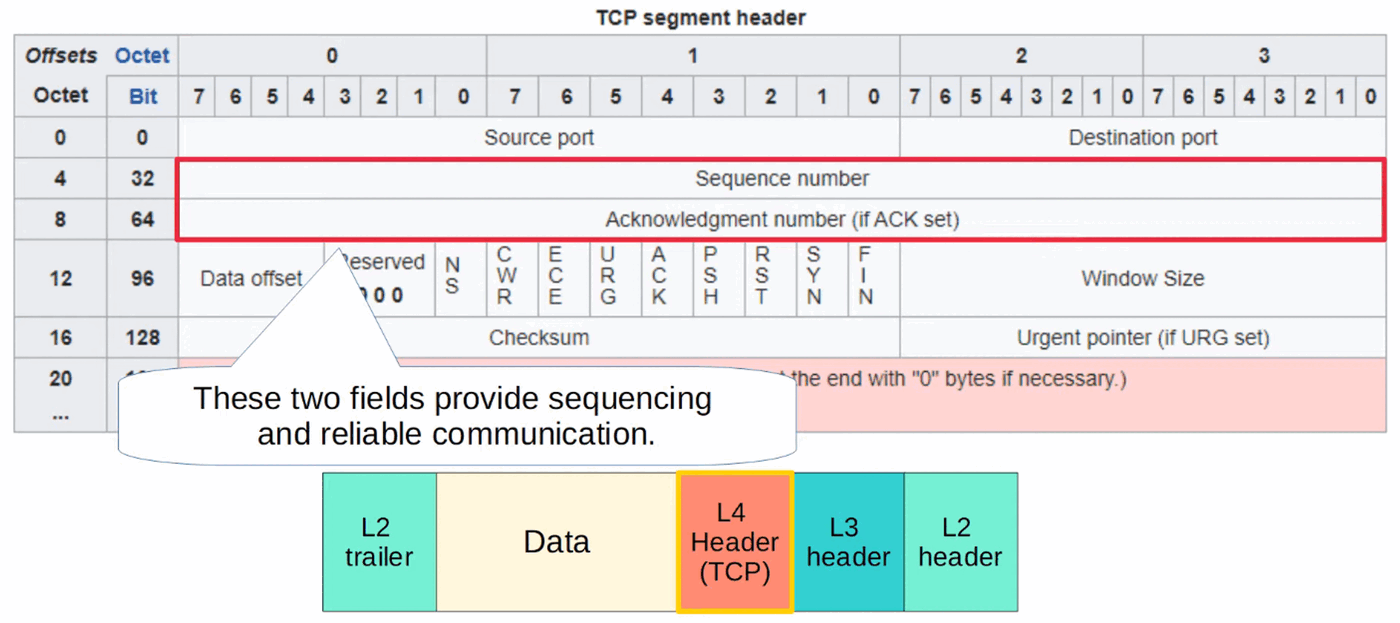
\includegraphics[keepaspectratio,alt={image}]{images/31-tcp-and-udp/img-004.png}}
\end{figure}

\begin{figure}
\centering
\pandocbounded{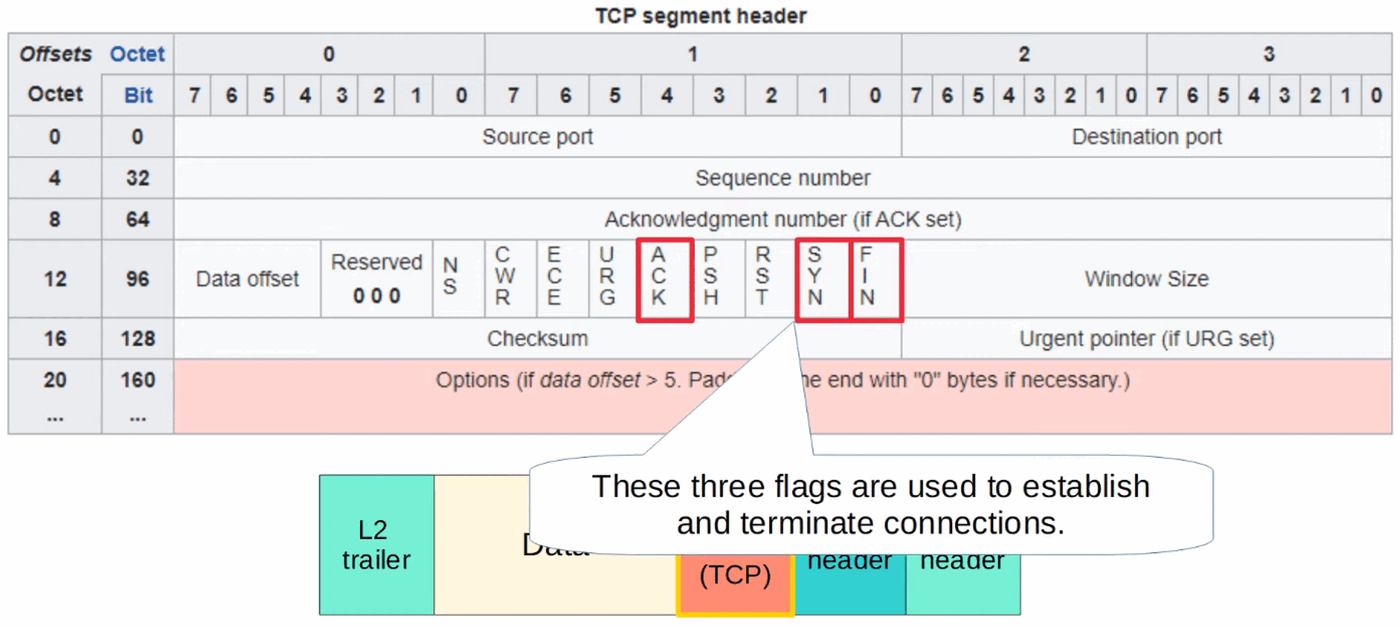
\includegraphics[keepaspectratio,alt={image}]{images/31-tcp-and-udp/img-005.png}}
\end{figure}

Establishing connections

\begin{figure}
\centering
\pandocbounded{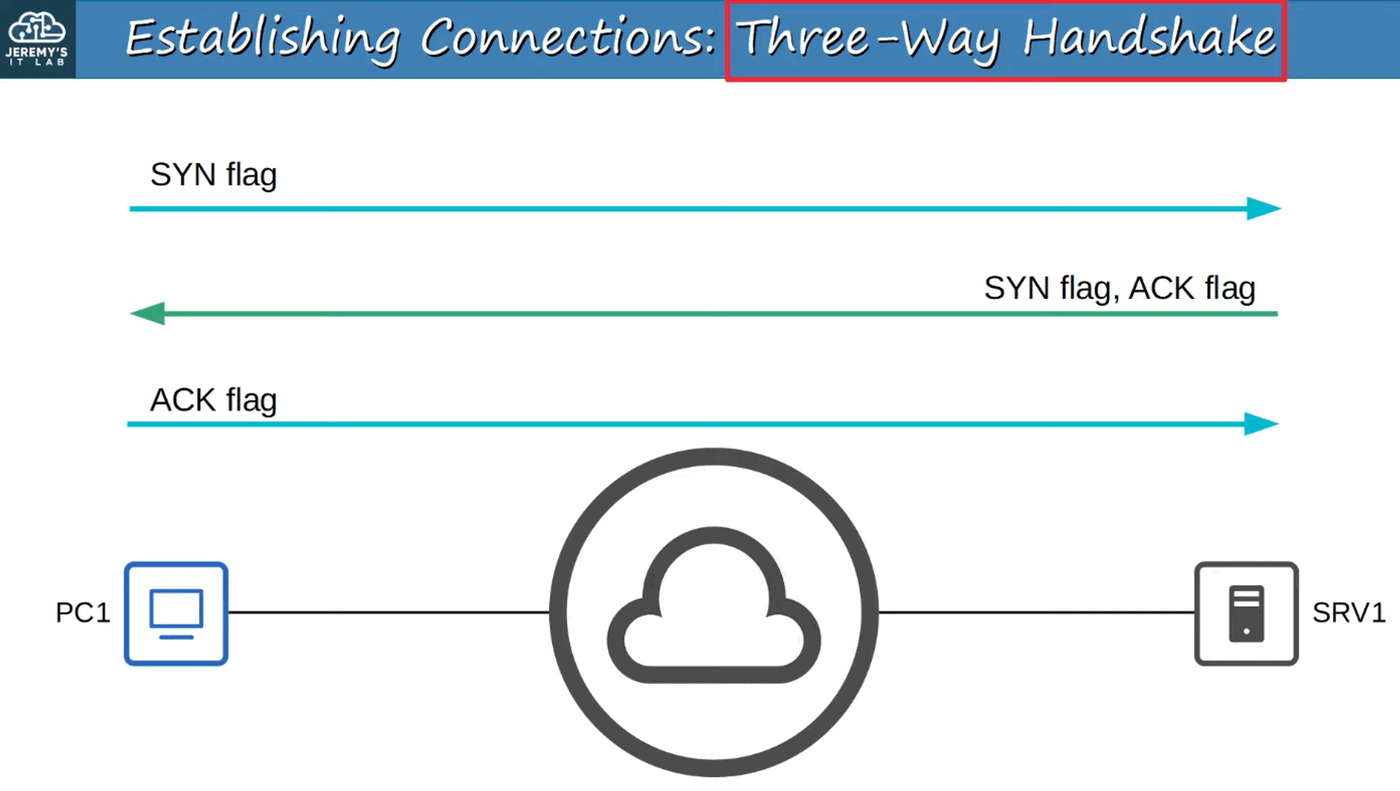
\includegraphics[keepaspectratio,alt={image}]{images/31-tcp-and-udp/img-006.png}}
\end{figure}

Terminating connections

\begin{figure}
\centering
\pandocbounded{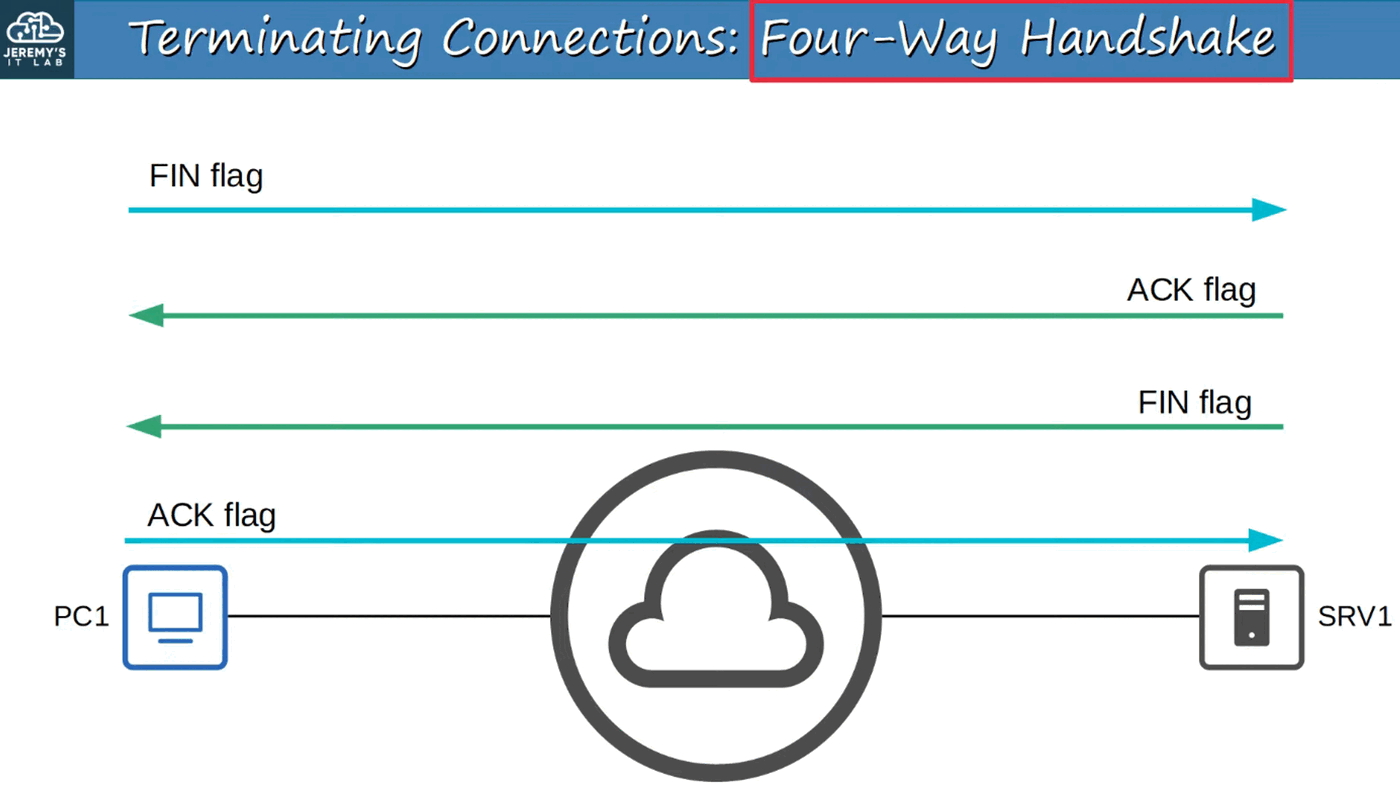
\includegraphics[keepaspectratio,alt={image}]{images/31-tcp-and-udp/img-007.png}}
\end{figure}

\begin{itemize}
\tightlist
\item
  TCP provides RELIABLE communication

  \begin{itemize}
  \tightlist
  \item
    The DESTINATION HOST must acknowledge that it RECEIVED each TCP
    SEGMENT (Layer 4 PDU)
  \item
    If a SEGMENT isn't ACKNOWLEDGED, it is sent again
  \end{itemize}
\end{itemize}

\begin{figure}
\centering
\pandocbounded{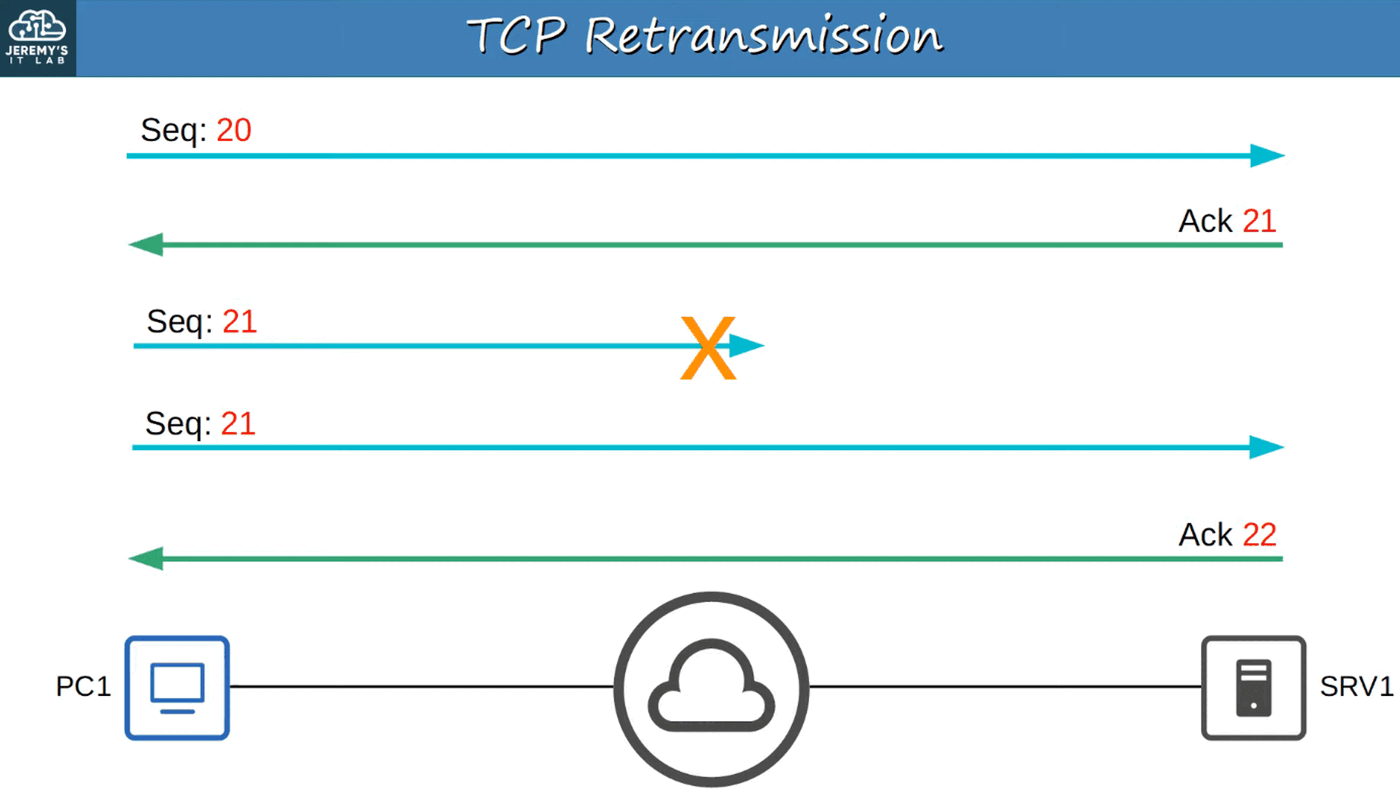
\includegraphics[keepaspectratio,alt={image}]{images/31-tcp-and-udp/img-008.png}}
\end{figure}

\begin{itemize}
\tightlist
\item
  TCP provides SEQUENCING

  \begin{itemize}
  \tightlist
  \item
    SEQUENCE numbers in the TCP HEADER allow DESTINATION HOSTS to put
    SEGMENTS in the correct ORDER even if they arrive out of ORDER
  \end{itemize}
\end{itemize}

\begin{figure}
\centering
\pandocbounded{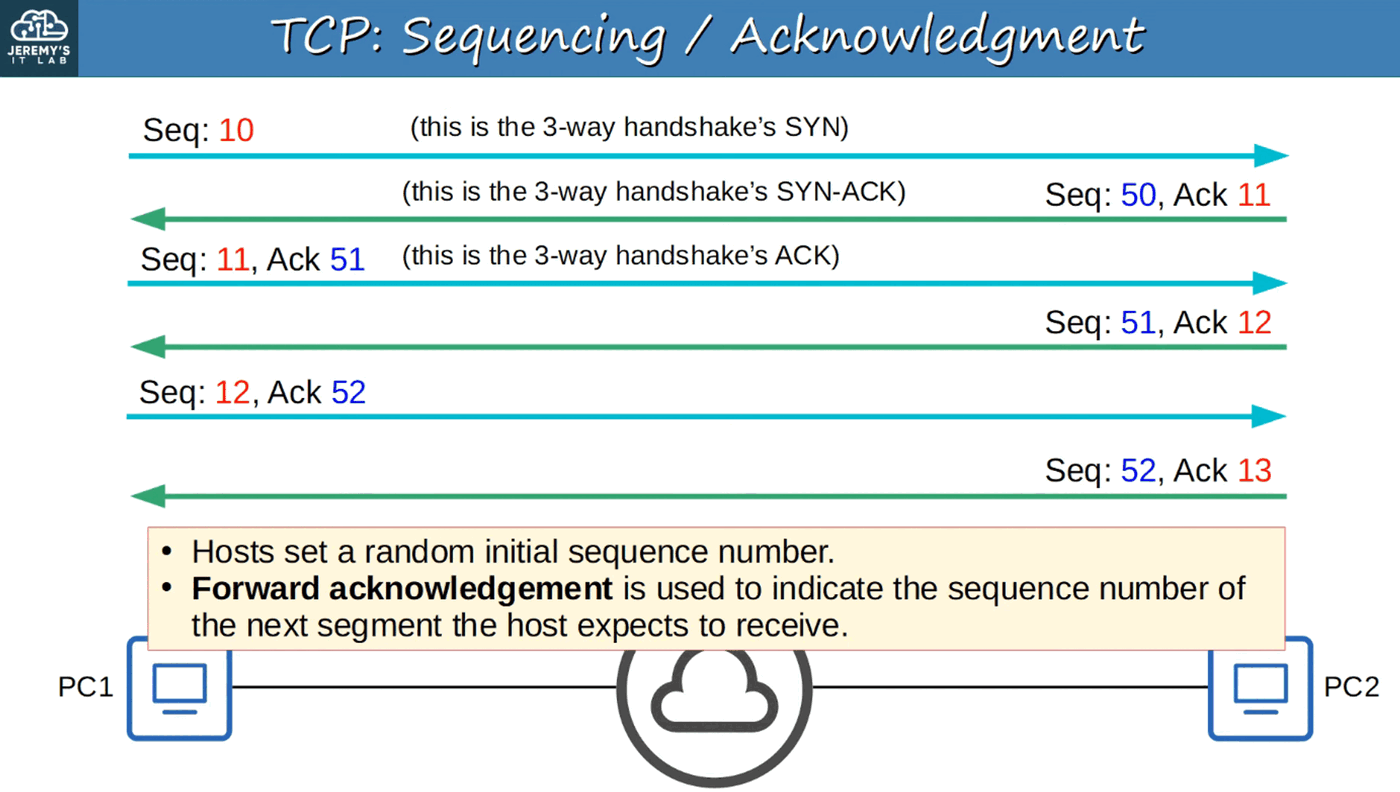
\includegraphics[keepaspectratio,alt={image}]{images/31-tcp-and-udp/img-009.png}}
\end{figure}

\begin{itemize}
\tightlist
\item
  TCP provides FLOW CONTROL

  \begin{itemize}
  \tightlist
  \item
    The DESTINATION HOST can tell the SOURCE HOST to increase / decrease
    the RATE that DATA is sent
  \end{itemize}
\end{itemize}

\begin{figure}
\centering
\pandocbounded{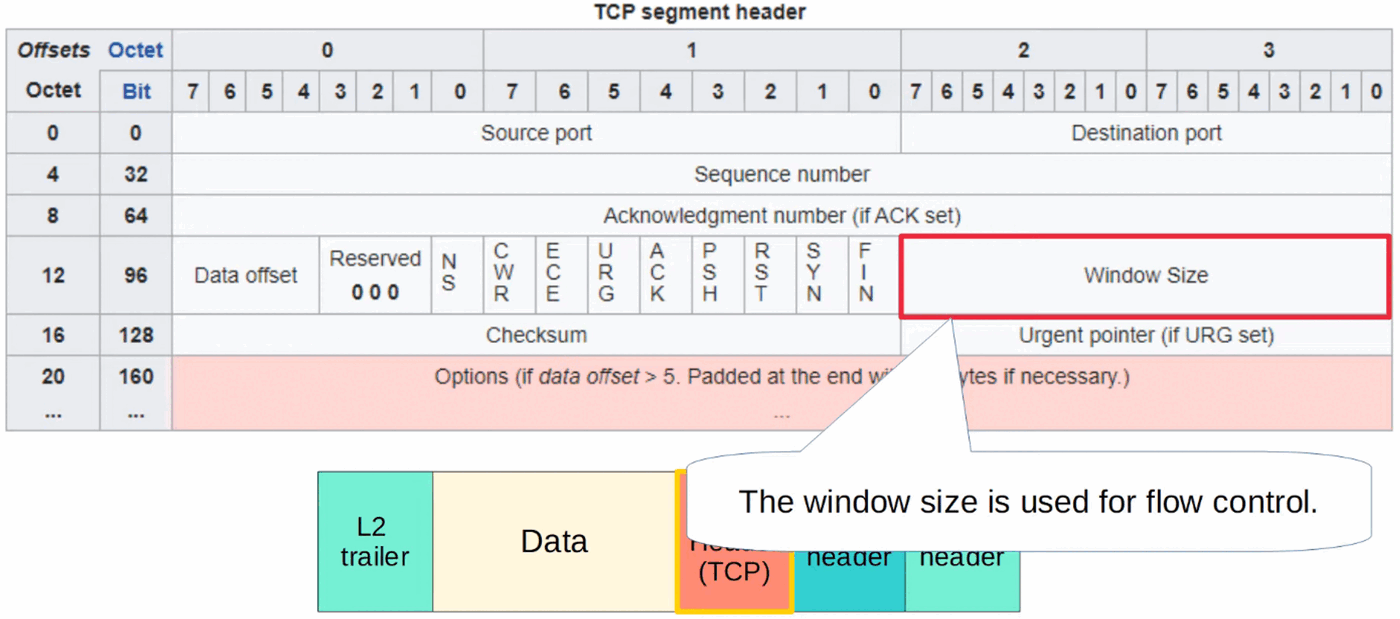
\includegraphics[keepaspectratio,alt={image}]{images/31-tcp-and-udp/img-010.png}}
\end{figure}

\begin{figure}
\centering
\pandocbounded{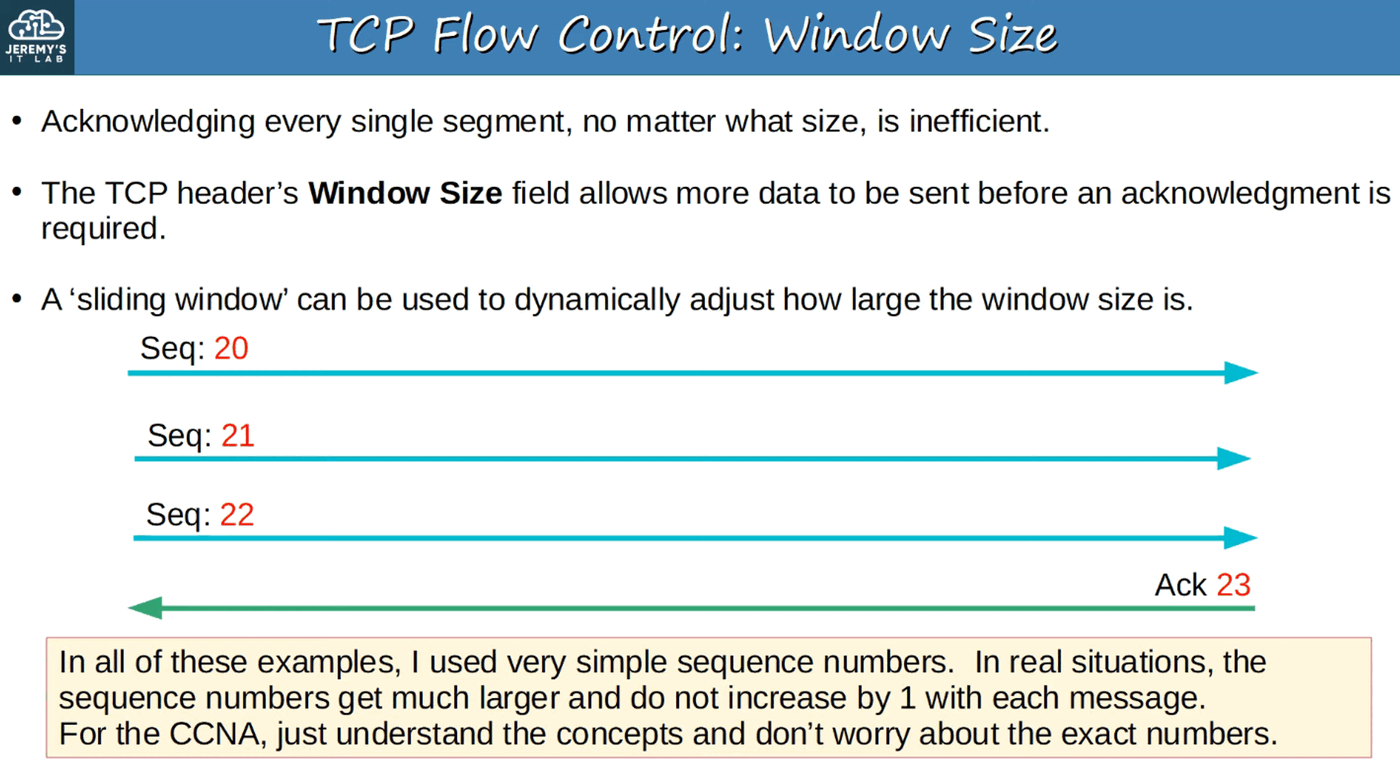
\includegraphics[keepaspectratio,alt={image}]{images/31-tcp-and-udp/img-011.png}}
\end{figure}

\section{UDP (User Datagram Protocol)}\label{udp-user-datagram-protocol}

\begin{figure}
\centering
\pandocbounded{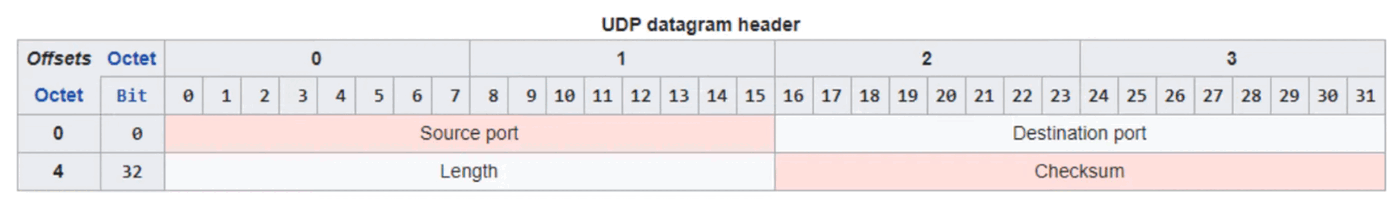
\includegraphics[keepaspectratio,alt={image}]{images/31-tcp-and-udp/img-012.png}}
\end{figure}

\begin{itemize}
\tightlist
\item
  UDP is NOT a CONNECTION-ORIENTED PROTOCOL

  \begin{itemize}
  \tightlist
  \item
    The SENDING HOST does NOT establish a CONNECTION with the
    DESTINATION HOST before sending DATA. The DATA is simply SENT
  \end{itemize}
\item
  UDP DOES NOT provide reliable COMMUNICATION

  \begin{itemize}
  \tightlist
  \item
    When UDP is used, ACKNOWLEDGEMENTS are NOT SENT for received
    SEGMENTS
  \item
    If a SEGMENT is LOST, UDP has no mechanism to re-TRASMIT it
  \item
    SEGMENTS are sent ``best-effort''
  \end{itemize}
\item
  UDP DOES NOT provide SEQUENCING

  \begin{itemize}
  \tightlist
  \item
    There is NO SEQUENCE NUMBER FIELD in the UDP header
  \item
    If SEGMENTS arrive out of order, UDP has no MECHANISM to put them
    back in ORDER
  \end{itemize}
\item
  UDP DOES NOT provide FLOW CONTROL

  \begin{itemize}
  \tightlist
  \item
    UDP has NO MECHANISM like TCP's WINDOW SIZE to control the flow of
    DATA
  \end{itemize}
\item
  UDP DOES provide ERROR CHECKING (via CHECKSUM)
\end{itemize}

\section{Comparing TCP and UDP}\label{comparing-tcp-and-udp}

Number of Fields in their Headers

\begin{figure}
\centering
\pandocbounded{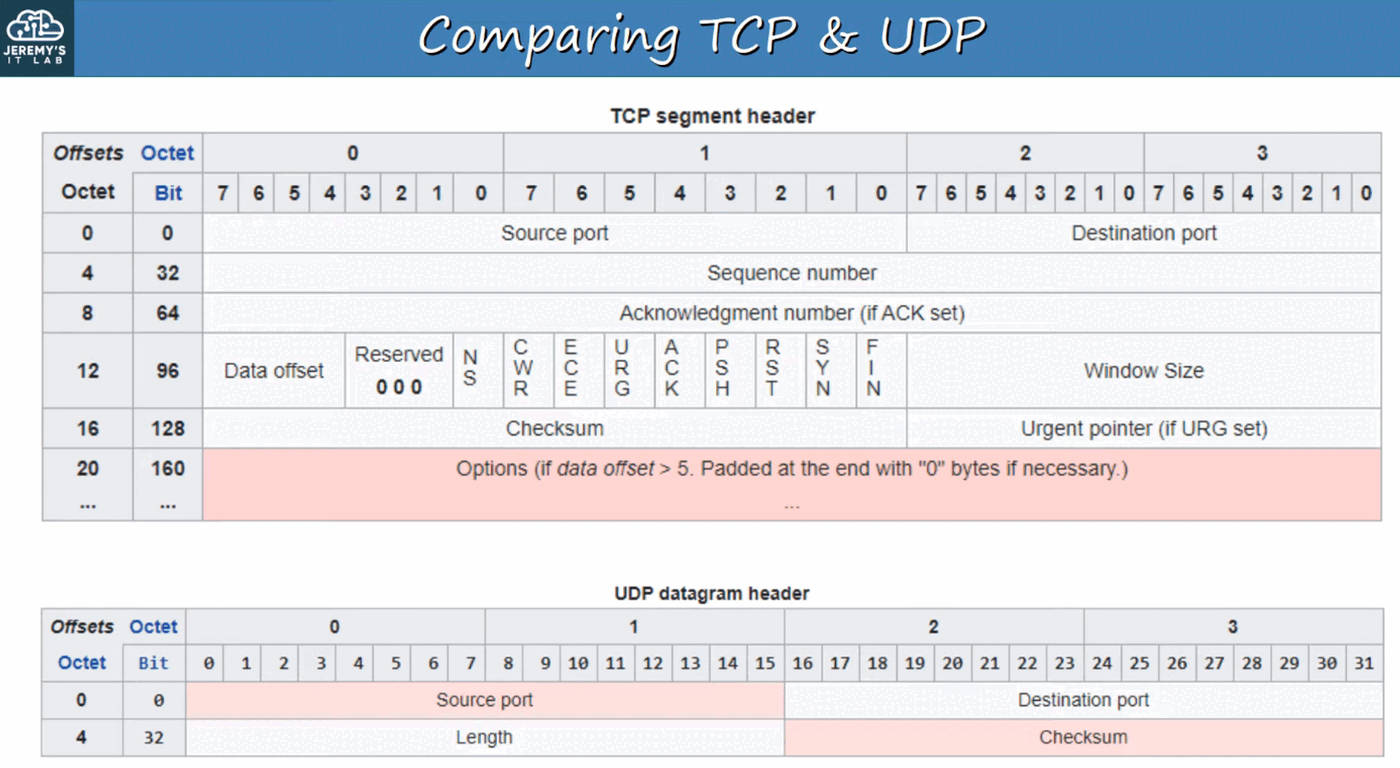
\includegraphics[keepaspectratio,alt={image}]{images/31-tcp-and-udp/img-013.png}}
\end{figure}

\begin{itemize}
\tightlist
\item
  TCP provides MORE FEATURES than UDP but at a COST of ADDITIONAL
  OVERHEAD
\item
  For applications that require RELIABLE communications (for example,
  downloading a file), TCP is PREFERRED
\item
  For applications, like real-time voice and video, UDP is preferred
\item
  There are SOME applications that use UDP, but provide RELIABILITY,
  etc. within the APPLICATION itself.
\item
  Some applications use BOTH TCP and UDP, depending on the situation.
\end{itemize}

\begin{figure}
\centering
\pandocbounded{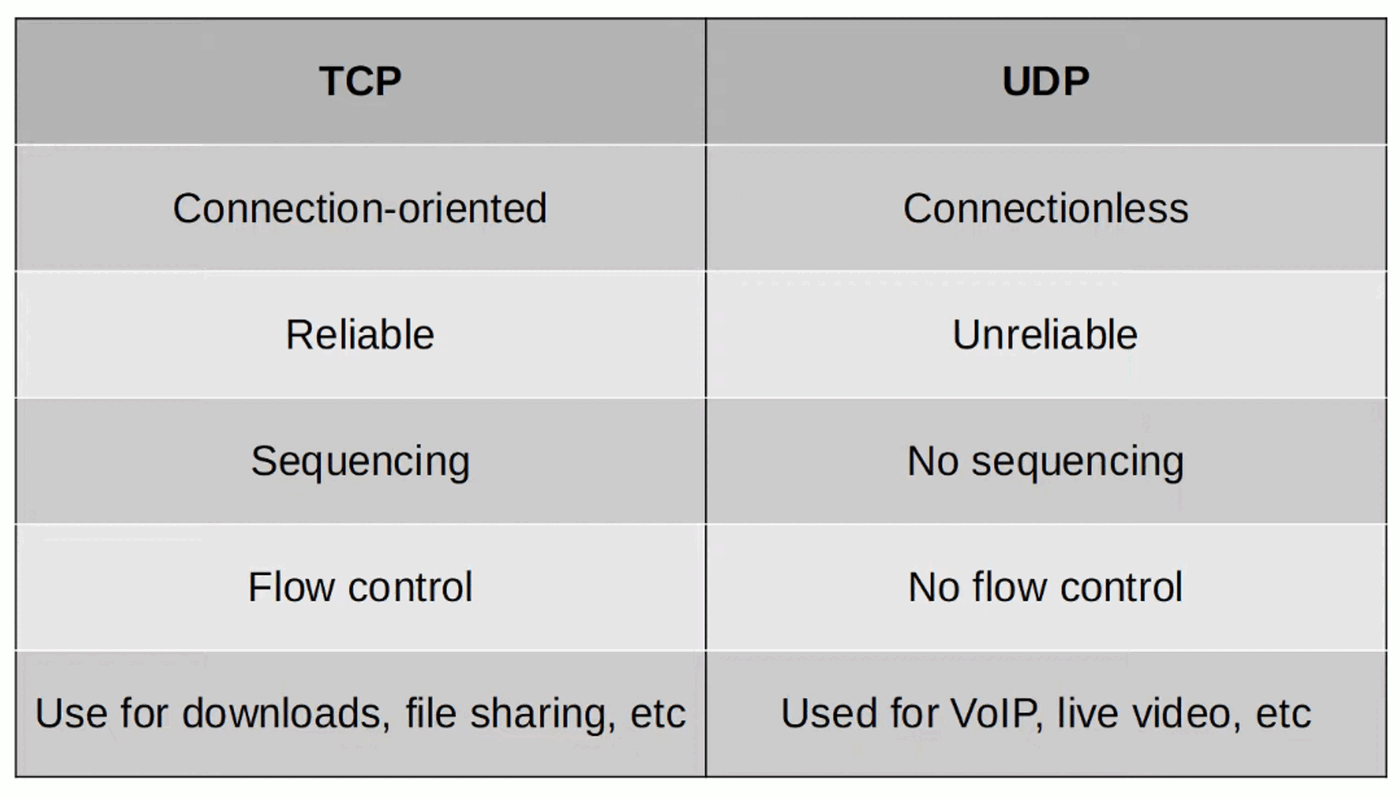
\includegraphics[keepaspectratio,alt={image}]{images/31-tcp-and-udp/img-014.png}}
\end{figure}

\section{Important Port Numbers}\label{important-port-numbers}

\begin{figure}
\centering
\pandocbounded{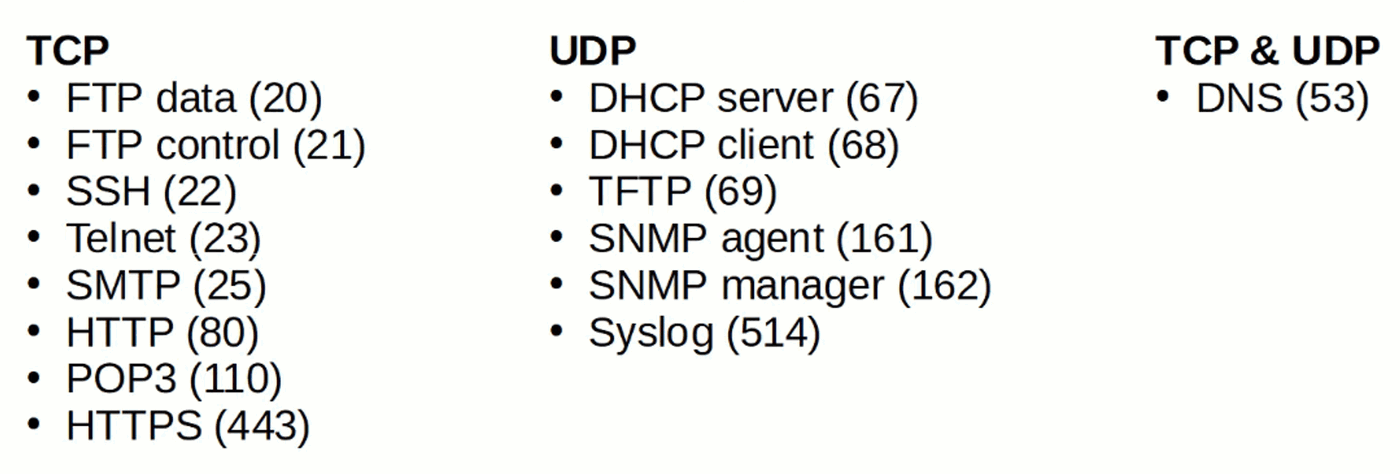
\includegraphics[keepaspectratio,alt={image}]{images/31-tcp-and-udp/img-015.png}}
\end{figure}
